We apply REFLOW to magnitude pruning (MP) and evaluate it across small, medium, and large architectures. The results highlight REFLOW’s consistently recovers performance in pruned networks, achieving state-of-the-art accuracy without requiring computationally expensive Hessian-based updates. By mitigating signal collapse, REFLOW enables the discovery of high-quality sparse subnetworks within the original parameter space.

\subsection{Performance on Small Architectures}
We begin by evaluating REFLOW on small architectures, namely ResNet-20~\cite{RESNET} pre-trained on CIFAR-10~\cite{CIFAR10} and MobileNet~\cite{MobileNet} pre-trained on ImageNet~\cite{ImageNet}, with less than 5 million parameters and comparing them to state-of-the-art one-shot pruning approaches, namely WF~\cite{WoodFisher}, CBS~\cite{CBS}, and CHITA~\cite{CHITA}. 

Table~\ref{tab:small_architectures_results} highlights REFLOW’s accuracy improvements across all sparsity levels. For ResNet-20, REFLOW restores accuracy to 49.16\% at 0.9 sparsity, outperforming CHITA (15.60\%) and MP (11.79\%). On MobileNet, REFLOW achieves 43.37\% accuracy at 0.8 sparsity, surpassing CHITA (29.78\%) and MP (0.11\%). 

\begin{table}[h]
    \small
    \setlength{\tabcolsep}{4pt} % Reduce column padding
    \caption{Performance of pruning methods on small architectures (ResNet-20 on CIFAR-10 and MobileNet on ImageNet) across varying sparsity levels. Sparsity values represent the fraction of weights pruned (e.g., 0.4 corresponds to 40\% pruning). The unpruned test accuracy for ResNet-20 and MobileNet are 91.57\% and 71.96\%, respectively. The best accuracy values are highlighted in bold. Weight update indicates whether a single-pass Hessian-based update is performed on unpruned weights post-pruning.}
    \label{tab:small_architectures_results}
    \centering
    \resizebox{0.7\columnwidth}{!}{%
    \begin{tabular}{cccccccc}
        \toprule
        Dataset & Network & Sparsity & MP & WF & CBS & CHITA & REFLOW \\
        \midrule
        \multirow{6}{*}{CIFAR-10} & \multirow{6}{*}{ResNet-20} 
        & 0.4 & 89.98 & 91.15 & 91.21 & 91.19 & \textbf{91.25} \\
        & & 0.5 & 88.44 & 90.23 & 90.58 & 90.60 & \textbf{90.66} \\
        & & 0.6 & 85.24 & 87.96 & 88.88 & 89.22 & \textbf{89.49} \\
        & & 0.7 & 78.79 & 81.05 & 81.84 & 84.12 & \textbf{86.65} \\
        & & 0.8 & 54.01 & 62.63 & 51.28 & 57.90 & \textbf{78.50} \\
        & & 0.9 & 11.79 & 11.49 & 13.68 & 15.60 & \textbf{49.16} \\
        \midrule
        \multirow{5}{*}{ImageNet} & \multirow{5}{*}{MobileNet} 
        & 0.4 & 69.16 & 71.15 & 71.45 & 71.50 & \textbf{71.59} \\
        & & 0.5 & 62.61 & 68.91 & 70.21 & 70.42 & \textbf{70.48} \\
        & & 0.6 & 41.94 & 60.90 & 66.37 & 67.30 & \textbf{67.83} \\
        & & 0.7 & 6.78 & 29.36 & 55.11 & 59.40 & \textbf{61.54} \\
        & & 0.8 & 0.11 & 0.24 & 16.38 & 29.78 & \textbf{43.37} \\
        \midrule
        Weight Update & - & - &  \xmark & \cmark & \cmark & \cmark & \xmark \\
        \bottomrule
    \end{tabular}
    }
\end{table}

\subsection{Scaling REFLOW to Medium-sized Architectures}
We next evaluate REFLOW on medium-sized architectures, namely ResNet-50 (ImageNet) with less than 25 million parameters. For this size, we compare REFLOW to CHITA and M-FAC~\cite{mfac}, as WF and CBS are computationally prohibitive.

Figure~\ref{fig:resnet50_results} shows that REFLOW outperforms CHITA and M-FAC across all sparsity levels. At high sparsities, REFLOW offer superior accuracy improvements without the overhead of Hessian-based updates. %These results demonstrate that REFLOW’s mitigation of signal collapse scales effectively to larger models, maintaining both efficiency and high accuracy.
\begin{figure}[h]
    \centering
    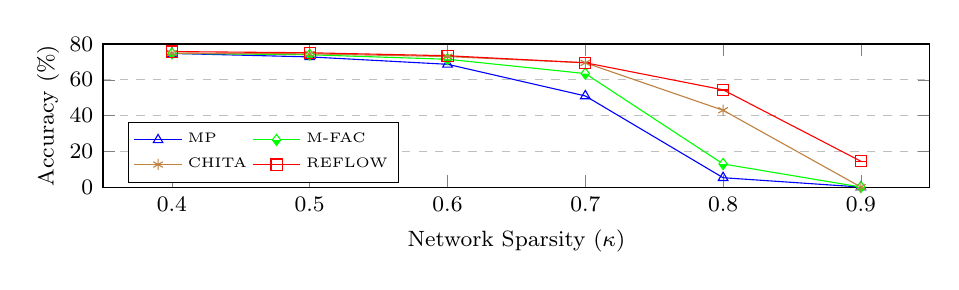
\begin{tikzpicture}
    \begin{axis}[
        width=10.5cm,
        height=0.15\textwidth,
        scale only axis,
        xlabel={Network Sparsity (\(\kappa\))},
        ylabel={Accuracy (\%)},
        xmin=0.35, xmax=0.95,
        ymin=0, ymax=80,
        ylabel near ticks,
        ylabel shift=-3pt,
        xtick={0.4,0.5,0.6,0.7,0.8,0.9},
        ymajorgrids=true,
        grid style=dashed,
        legend pos=south west,
        legend style={font=\tiny, cells={anchor=west}, inner sep=2pt, legend columns=2},
        tick label style={font=\footnotesize},
        label style={font=\footnotesize},
        legend cell align=left,
        mark options={scale=1},
        cycle list name=color list
    ]

    \addplot[color=blue,mark=triangle] coordinates {
        (0.40,74.74)
        (0.50,72.81) (0.60,68.68) 
        (0.70,51) (0.80,5.318) 
        (0.90,0.1)
    };
    \addlegendentry{MP}

    \addplot[color=green,mark=halfdiamond*] coordinates {
        (0.40,74.8)
        (0.50,74) (0.60,71.5) 
        (0.70,63.5) (0.80,13) 
        (0.90,0.1)
    };
    \addlegendentry{M-FAC}

    \addplot[color=brown,mark=asterisk] coordinates {
        (0.40,74.9)
        (0.50,74.5) (0.60,73) 
        (0.70,69.5) (0.80,43) 
        (0.90,0.1)
    };
    \addlegendentry{CHITA}

    \addplot[color=red,mark=square, error bars/.cd, y dir=both, y explicit] 
    coordinates {
        (0.40,75.788) +- (0,0.04)
        (0.50,75.12) +- (0,0.03)
        (0.60,73.466) +- (0,0.01)
        (0.70,69.55) +- (0,0.08)
        (0.80,54.412) +- (0,0.19)
        (0.90,14.506) +- (0,0.04)
    };
    \addlegendentry{REFLOW}

    \end{axis}
    \end{tikzpicture}
    \caption{Comparison of test accuracy for varying sparsities across pruning techniques for ResNet-50 on ImageNet. REFLOW outperforms CHITA, M-FAC, and MP consistently.}
    \label{fig:resnet50_results}
\end{figure}

\subsection{Scaling REFLOW to Large Architectures}
Finally, we consider large architectures, namely ResNet-101, ResNet-152, RegNetX-32GF (with nearly 107 million parameters), and ResNeXt-101 (64x4d) that has over 45 million parameters. These models pose significant challenges for pruning, particularly for CHITA as it relies on memory- and computation-intensive second-order approximations.
Figure~\ref{fig:large_architectures} shows that REFLOW delivers up to 74.8\% accuracy gains over MP on ImageNet. For instance, on ResNet-101, REFLOW restores accuracy from 4.1\% (MP) to 64.1\%. On ResNet-152, REFLOW achieves 68.2\% accuracy, compared to just 0.9\% for MP. Similar gains are observed for RegNetX-32GF, where REFLOW achieves 73.0\% accuracy, and for ResNeXt-101, where it achieves 78.9\%, outperforming MP. 

\begin{figure}[h]
    \centering
    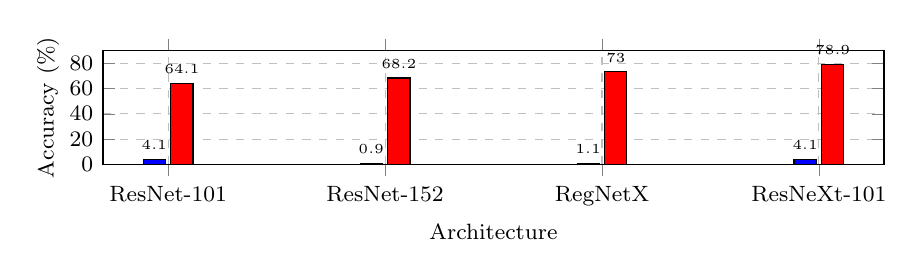
\begin{tikzpicture}
    \begin{axis}[
        width=11.5cm,
        height=0.25\textwidth,
        ybar,
        bar width=8pt,
        xlabel={Architecture},
        ylabel={\footnotesize Accuracy (\%)},
        ylabel style={font=\footnotesize}, % Apply tiny font to the ylabel
        ymin=0, ymax=90,
        xtick=data,
        xticklabel style={font=\footnotesize}, % Decreased font size for x-labels
        symbolic x coords={ResNet-101, ResNet-152, RegNetX, ResNeXt-101},
        grid=both,
        grid style=dashed,
        ymajorgrids=true,
        tick label style={font=\footnotesize}, % Set tick label font to tiny
        label style={font=\footnotesize}, % General label font size
        ylabel near ticks,
        ylabel shift=-3pt,
        legend style={font=\footnotesize, cells={anchor=west}, inner sep=2pt, legend columns=1, at={(0.5,1.05)}, anchor=south}, % Adjust legend style
        nodes near coords,
        every node near coord/.append style={font=\fontsize{0.1}{0.1}\selectfont} % Nodes near bars are tiny
    ]

    % MP Accuracy
    \addplot[fill=blue] coordinates {
        (ResNet-101, 4.1)
        (ResNet-152, 0.9)
        (RegNetX, 1.1)
        (ResNeXt-101, 4.1)
    };
    % \addlegendentry{MP}

    % REFLOW Accuracy
    \addplot[fill=red] coordinates {
        (ResNet-101, 64.1)
        (ResNet-152, 68.2)
        (RegNetX, 73.0)
        (ResNeXt-101, 78.9)
    };
    % \addlegendentry{REFLOW}

    \end{axis}
    \end{tikzpicture}
    \caption{Accuracy comparison of MP (blue) and REFLOW applied to MP (red) at 80\% sparsity for large architectures pre-trained on ImageNet. REFLOW mitigates signal collapse and restores accuracy.}
    \label{fig:large_architectures}
\end{figure}



\subsection{Convergence with REFLOW}
Building on the results in Table~\ref{tab:small_architectures_results}, we evaluate the impact of REFLOW across pruning methods with varying complexities: MP, CHITA-S (selection-only), and CHITA (selection with Hessian-based updates). CHITA updates the unpruned weights using second-order information, while CHITA-S applies the same selection criteria without weight updates. This distinction isolates the role of weight updates and quantifies whether REFLOW can compensate for their absence.

Figure~\ref{fig:reflow_convergence} shows that REFLOW bridges the performance gap between MP, CHITA-S, and CHITA. REFLOW enables simpler selection based approaches like MP and CHITA-S to achieve comparable accuracy as CHITA (Hessian-based weight updates) although the latter is computationally intensive. This highlights that mitigating signal collapse, rather than employing complex pruning selection heuristics, is the key to recovering performance in one-shot pruned networks.




\begin{figure}[h]
    \centering
    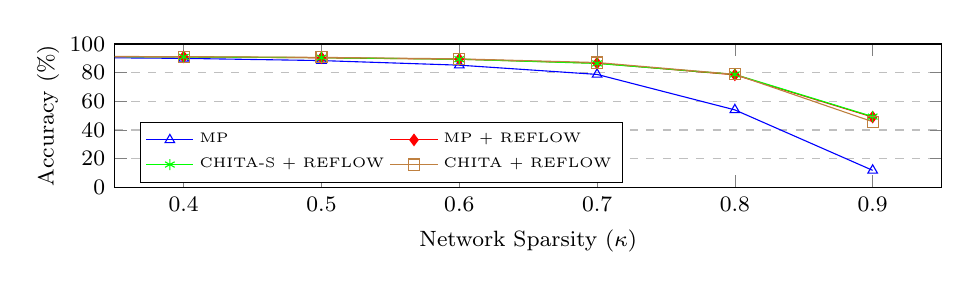
\begin{tikzpicture}
    \begin{axis}[
        width=10.5cm,
        height=0.15\textwidth,
        scale only axis,
        xlabel={Network Sparsity (\(\kappa\))},
        ylabel={Accuracy (\%)},
        xmin=0.35, xmax=0.95,
        ymin=0, ymax=100,
        ylabel near ticks,
        ylabel shift=-3pt,
        xtick={0.4,0.5,0.6,0.7,0.8,0.9},
        ymajorgrids=true,
        grid style=dashed,
        legend pos=south west,
        legend style={font=\tiny, cells={anchor=west}, inner sep=2pt, legend columns=2},
        tick label style={font=\footnotesize},
        label style={font=\footnotesize},
        legend cell align=left,
        mark options={scale=1},
        cycle list name=color list
    ]

    % MP (Blue)
    \addplot[color=blue,mark=triangle] coordinates {
        (0.3,90.77) (0.4,89.98) (0.5,88.44) 
        (0.6,85.24) (0.7,78.79) (0.8,54.01) 
        (0.9,11.79)
    };
    \addlegendentry{MP}

    % MP + REFLOW (Red)
    \addplot[color=red,mark=diamond*] coordinates {
        (0.3,91.41) (0.4,91.05) (0.5,90.39) 
        (0.6,89.38) (0.7,86.65) (0.8,78.5) 
        (0.9,49.0)
    };
    \addlegendentry{MP + REFLOW}

    % CHITA-S + REFLOW (Green)
    \addplot[color=green,mark=asterisk] coordinates {
        (0.3,91.37) (0.4,91.0) (0.5,90.45) 
        (0.6,89.41) (0.7,86.45) (0.8,78.79) 
        (0.9,49.35)
    };
    \addlegendentry{CHITA-S + REFLOW}

    % CHITA-U + REFLOW (Brown)
    \addplot[color=brown,mark=square, error bars/.cd, y dir=both, y explicit] 
    coordinates {
        (0.3,91.43) (0.4,91.17) (0.5,90.68) 
        (0.6,89.64) (0.7,87.08) (0.8,78.84) 
        (0.9,45.76)
    };
    \addlegendentry{CHITA + REFLOW}

    \end{axis}
    \end{tikzpicture}
    \caption{Comparison of test accuracy vs. sparsity for ResNet-20 on CIFAR-10.}
    \label{fig:reflow_convergence}
\end{figure}


